
% Default to the notebook output style

    


% Inherit from the specified cell style.




    
\documentclass[11pt]{article}

    
    
    \usepackage[T1]{fontenc}
    % Nicer default font (+ math font) than Computer Modern for most use cases
    \usepackage{mathpazo}

    % Basic figure setup, for now with no caption control since it's done
    % automatically by Pandoc (which extracts ![](path) syntax from Markdown).
    \usepackage{graphicx}
    % We will generate all images so they have a width \maxwidth. This means
    % that they will get their normal width if they fit onto the page, but
    % are scaled down if they would overflow the margins.
    \makeatletter
    \def\maxwidth{\ifdim\Gin@nat@width>\linewidth\linewidth
    \else\Gin@nat@width\fi}
    \makeatother
    \let\Oldincludegraphics\includegraphics
    % Set max figure width to be 80% of text width, for now hardcoded.
  
    % Ensure that by default, figures have no caption (until we provide a
    % proper Figure object with a Caption API and a way to capture that
    % in the conversion process - todo).
    \usepackage{caption}
    \DeclareCaptionLabelFormat{nolabel}{}
    \captionsetup{labelformat=nolabel}

    \usepackage{adjustbox} % Used to constrain images to a maximum size 
    \usepackage{xcolor} % Allow colors to be defined
    \usepackage{enumerate} % Needed for markdown enumerations to work
    \usepackage{geometry} % Used to adjust the document margins
    \usepackage{amsmath} % Equations
    \usepackage{amssymb} % Equations
    \usepackage{textcomp} % defines textquotesingle
    % Hack from http://tex.stackexchange.com/a/47451/13684:
    \AtBeginDocument{%
        \def\PYZsq{\textquotesingle}% Upright quotes in Pygmentized code
    }
    \usepackage{upquote} % Upright quotes for verbatim code
    \usepackage{eurosym} % defines \euro
    \usepackage[mathletters]{ucs} % Extended unicode (utf-8) support
    \usepackage[utf8x]{inputenc} % Allow utf-8 characters in the tex document
    \usepackage{fancyvrb} % verbatim replacement that allows latex
    \usepackage{grffile} % extends the file name processing of package graphics 
                         % to support a larger range 
    % The hyperref package gives us a pdf with properly built
    % internal navigation ('pdf bookmarks' for the table of contents,
    % internal cross-reference links, web links for URLs, etc.)
    \usepackage{hyperref}
    \usepackage{longtable} % longtable support required by pandoc >1.10
    \usepackage{booktabs}  % table support for pandoc > 1.12.2
    \usepackage[inline]{enumitem} % IRkernel/repr support (it uses the enumerate* environment)
    \usepackage[normalem]{ulem} % ulem is needed to support strikethroughs (\sout)
                                % normalem makes italics be italics, not underlines
    \usepackage{mathrsfs}
    

    
    
    % Colors for the hyperref package
    \definecolor{urlcolor}{rgb}{0,.145,.698}
    \definecolor{linkcolor}{rgb}{.71,0.21,0.01}
    \definecolor{citecolor}{rgb}{.12,.54,.11}

    % ANSI colors
    \definecolor{ansi-black}{HTML}{3E424D}
    \definecolor{ansi-black-intense}{HTML}{282C36}
    \definecolor{ansi-red}{HTML}{E75C58}
    \definecolor{ansi-red-intense}{HTML}{B22B31}
    \definecolor{ansi-green}{HTML}{00A250}
    \definecolor{ansi-green-intense}{HTML}{007427}
    \definecolor{ansi-yellow}{HTML}{DDB62B}
    \definecolor{ansi-yellow-intense}{HTML}{B27D12}
    \definecolor{ansi-blue}{HTML}{208FFB}
    \definecolor{ansi-blue-intense}{HTML}{0065CA}
    \definecolor{ansi-magenta}{HTML}{D160C4}
    \definecolor{ansi-magenta-intense}{HTML}{A03196}
    \definecolor{ansi-cyan}{HTML}{60C6C8}
    \definecolor{ansi-cyan-intense}{HTML}{258F8F}
    \definecolor{ansi-white}{HTML}{C5C1B4}
    \definecolor{ansi-white-intense}{HTML}{A1A6B2}
    \definecolor{ansi-default-inverse-fg}{HTML}{FFFFFF}
    \definecolor{ansi-default-inverse-bg}{HTML}{000000}

    % commands and environments needed by pandoc snippets
    % extracted from the output of `pandoc -s`
    \providecommand{\tightlist}{%
      \setlength{\itemsep}{0pt}\setlength{\parskip}{0pt}}
    \DefineVerbatimEnvironment{Highlighting}{Verbatim}{commandchars=\\\{\}}
    % Add ',fontsize=\small' for more characters per line
    \newenvironment{Shaded}{}{}
    \newcommand{\KeywordTok}[1]{\textcolor[rgb]{0.00,0.44,0.13}{\textbf{{#1}}}}
    \newcommand{\DataTypeTok}[1]{\textcolor[rgb]{0.56,0.13,0.00}{{#1}}}
    \newcommand{\DecValTok}[1]{\textcolor[rgb]{0.25,0.63,0.44}{{#1}}}
    \newcommand{\BaseNTok}[1]{\textcolor[rgb]{0.25,0.63,0.44}{{#1}}}
    \newcommand{\FloatTok}[1]{\textcolor[rgb]{0.25,0.63,0.44}{{#1}}}
    \newcommand{\CharTok}[1]{\textcolor[rgb]{0.25,0.44,0.63}{{#1}}}
    \newcommand{\StringTok}[1]{\textcolor[rgb]{0.25,0.44,0.63}{{#1}}}
    \newcommand{\CommentTok}[1]{\textcolor[rgb]{0.38,0.63,0.69}{\textit{{#1}}}}
    \newcommand{\OtherTok}[1]{\textcolor[rgb]{0.00,0.44,0.13}{{#1}}}
    \newcommand{\AlertTok}[1]{\textcolor[rgb]{1.00,0.00,0.00}{\textbf{{#1}}}}
    \newcommand{\FunctionTok}[1]{\textcolor[rgb]{0.02,0.16,0.49}{{#1}}}
    \newcommand{\RegionMarkerTok}[1]{{#1}}
    \newcommand{\ErrorTok}[1]{\textcolor[rgb]{1.00,0.00,0.00}{\textbf{{#1}}}}
    \newcommand{\NormalTok}[1]{{#1}}
    
    % Additional commands for more recent versions of Pandoc
    \newcommand{\ConstantTok}[1]{\textcolor[rgb]{0.53,0.00,0.00}{{#1}}}
    \newcommand{\SpecialCharTok}[1]{\textcolor[rgb]{0.25,0.44,0.63}{{#1}}}
    \newcommand{\VerbatimStringTok}[1]{\textcolor[rgb]{0.25,0.44,0.63}{{#1}}}
    \newcommand{\SpecialStringTok}[1]{\textcolor[rgb]{0.73,0.40,0.53}{{#1}}}
    \newcommand{\ImportTok}[1]{{#1}}
    \newcommand{\DocumentationTok}[1]{\textcolor[rgb]{0.73,0.13,0.13}{\textit{{#1}}}}
    \newcommand{\AnnotationTok}[1]{\textcolor[rgb]{0.38,0.63,0.69}{\textbf{\textit{{#1}}}}}
    \newcommand{\CommentVarTok}[1]{\textcolor[rgb]{0.38,0.63,0.69}{\textbf{\textit{{#1}}}}}
    \newcommand{\VariableTok}[1]{\textcolor[rgb]{0.10,0.09,0.49}{{#1}}}
    \newcommand{\ControlFlowTok}[1]{\textcolor[rgb]{0.00,0.44,0.13}{\textbf{{#1}}}}
    \newcommand{\OperatorTok}[1]{\textcolor[rgb]{0.40,0.40,0.40}{{#1}}}
    \newcommand{\BuiltInTok}[1]{{#1}}
    \newcommand{\ExtensionTok}[1]{{#1}}
    \newcommand{\PreprocessorTok}[1]{\textcolor[rgb]{0.74,0.48,0.00}{{#1}}}
    \newcommand{\AttributeTok}[1]{\textcolor[rgb]{0.49,0.56,0.16}{{#1}}}
    \newcommand{\InformationTok}[1]{\textcolor[rgb]{0.38,0.63,0.69}{\textbf{\textit{{#1}}}}}
    \newcommand{\WarningTok}[1]{\textcolor[rgb]{0.38,0.63,0.69}{\textbf{\textit{{#1}}}}}
    
    
    % Define a nice break command that doesn't care if a line doesn't already
    % exist.
    \def\br{\hspace*{\fill} \\* }
    % Math Jax compatibility definitions
    \def\gt{>}
    \def\lt{<}
    \let\Oldtex\TeX
    \let\Oldlatex\LaTeX
    \renewcommand{\TeX}{\textrm{\Oldtex}}
    \renewcommand{\LaTeX}{\textrm{\Oldlatex}}
    % Document parameters
    % Document title
    \title{lecture\_10}
    
    
    
    
    

    % Pygments definitions
    
\makeatletter
\def\PY@reset{\let\PY@it=\relax \let\PY@bf=\relax%
    \let\PY@ul=\relax \let\PY@tc=\relax%
    \let\PY@bc=\relax \let\PY@ff=\relax}
\def\PY@tok#1{\csname PY@tok@#1\endcsname}
\def\PY@toks#1+{\ifx\relax#1\empty\else%
    \PY@tok{#1}\expandafter\PY@toks\fi}
\def\PY@do#1{\PY@bc{\PY@tc{\PY@ul{%
    \PY@it{\PY@bf{\PY@ff{#1}}}}}}}
\def\PY#1#2{\PY@reset\PY@toks#1+\relax+\PY@do{#2}}

\expandafter\def\csname PY@tok@w\endcsname{\def\PY@tc##1{\textcolor[rgb]{0.73,0.73,0.73}{##1}}}
\expandafter\def\csname PY@tok@c\endcsname{\let\PY@it=\textit\def\PY@tc##1{\textcolor[rgb]{0.25,0.50,0.50}{##1}}}
\expandafter\def\csname PY@tok@cp\endcsname{\def\PY@tc##1{\textcolor[rgb]{0.74,0.48,0.00}{##1}}}
\expandafter\def\csname PY@tok@k\endcsname{\let\PY@bf=\textbf\def\PY@tc##1{\textcolor[rgb]{0.00,0.50,0.00}{##1}}}
\expandafter\def\csname PY@tok@kp\endcsname{\def\PY@tc##1{\textcolor[rgb]{0.00,0.50,0.00}{##1}}}
\expandafter\def\csname PY@tok@kt\endcsname{\def\PY@tc##1{\textcolor[rgb]{0.69,0.00,0.25}{##1}}}
\expandafter\def\csname PY@tok@o\endcsname{\def\PY@tc##1{\textcolor[rgb]{0.40,0.40,0.40}{##1}}}
\expandafter\def\csname PY@tok@ow\endcsname{\let\PY@bf=\textbf\def\PY@tc##1{\textcolor[rgb]{0.67,0.13,1.00}{##1}}}
\expandafter\def\csname PY@tok@nb\endcsname{\def\PY@tc##1{\textcolor[rgb]{0.00,0.50,0.00}{##1}}}
\expandafter\def\csname PY@tok@nf\endcsname{\def\PY@tc##1{\textcolor[rgb]{0.00,0.00,1.00}{##1}}}
\expandafter\def\csname PY@tok@nc\endcsname{\let\PY@bf=\textbf\def\PY@tc##1{\textcolor[rgb]{0.00,0.00,1.00}{##1}}}
\expandafter\def\csname PY@tok@nn\endcsname{\let\PY@bf=\textbf\def\PY@tc##1{\textcolor[rgb]{0.00,0.00,1.00}{##1}}}
\expandafter\def\csname PY@tok@ne\endcsname{\let\PY@bf=\textbf\def\PY@tc##1{\textcolor[rgb]{0.82,0.25,0.23}{##1}}}
\expandafter\def\csname PY@tok@nv\endcsname{\def\PY@tc##1{\textcolor[rgb]{0.10,0.09,0.49}{##1}}}
\expandafter\def\csname PY@tok@no\endcsname{\def\PY@tc##1{\textcolor[rgb]{0.53,0.00,0.00}{##1}}}
\expandafter\def\csname PY@tok@nl\endcsname{\def\PY@tc##1{\textcolor[rgb]{0.63,0.63,0.00}{##1}}}
\expandafter\def\csname PY@tok@ni\endcsname{\let\PY@bf=\textbf\def\PY@tc##1{\textcolor[rgb]{0.60,0.60,0.60}{##1}}}
\expandafter\def\csname PY@tok@na\endcsname{\def\PY@tc##1{\textcolor[rgb]{0.49,0.56,0.16}{##1}}}
\expandafter\def\csname PY@tok@nt\endcsname{\let\PY@bf=\textbf\def\PY@tc##1{\textcolor[rgb]{0.00,0.50,0.00}{##1}}}
\expandafter\def\csname PY@tok@nd\endcsname{\def\PY@tc##1{\textcolor[rgb]{0.67,0.13,1.00}{##1}}}
\expandafter\def\csname PY@tok@s\endcsname{\def\PY@tc##1{\textcolor[rgb]{0.73,0.13,0.13}{##1}}}
\expandafter\def\csname PY@tok@sd\endcsname{\let\PY@it=\textit\def\PY@tc##1{\textcolor[rgb]{0.73,0.13,0.13}{##1}}}
\expandafter\def\csname PY@tok@si\endcsname{\let\PY@bf=\textbf\def\PY@tc##1{\textcolor[rgb]{0.73,0.40,0.53}{##1}}}
\expandafter\def\csname PY@tok@se\endcsname{\let\PY@bf=\textbf\def\PY@tc##1{\textcolor[rgb]{0.73,0.40,0.13}{##1}}}
\expandafter\def\csname PY@tok@sr\endcsname{\def\PY@tc##1{\textcolor[rgb]{0.73,0.40,0.53}{##1}}}
\expandafter\def\csname PY@tok@ss\endcsname{\def\PY@tc##1{\textcolor[rgb]{0.10,0.09,0.49}{##1}}}
\expandafter\def\csname PY@tok@sx\endcsname{\def\PY@tc##1{\textcolor[rgb]{0.00,0.50,0.00}{##1}}}
\expandafter\def\csname PY@tok@m\endcsname{\def\PY@tc##1{\textcolor[rgb]{0.40,0.40,0.40}{##1}}}
\expandafter\def\csname PY@tok@gh\endcsname{\let\PY@bf=\textbf\def\PY@tc##1{\textcolor[rgb]{0.00,0.00,0.50}{##1}}}
\expandafter\def\csname PY@tok@gu\endcsname{\let\PY@bf=\textbf\def\PY@tc##1{\textcolor[rgb]{0.50,0.00,0.50}{##1}}}
\expandafter\def\csname PY@tok@gd\endcsname{\def\PY@tc##1{\textcolor[rgb]{0.63,0.00,0.00}{##1}}}
\expandafter\def\csname PY@tok@gi\endcsname{\def\PY@tc##1{\textcolor[rgb]{0.00,0.63,0.00}{##1}}}
\expandafter\def\csname PY@tok@gr\endcsname{\def\PY@tc##1{\textcolor[rgb]{1.00,0.00,0.00}{##1}}}
\expandafter\def\csname PY@tok@ge\endcsname{\let\PY@it=\textit}
\expandafter\def\csname PY@tok@gs\endcsname{\let\PY@bf=\textbf}
\expandafter\def\csname PY@tok@gp\endcsname{\let\PY@bf=\textbf\def\PY@tc##1{\textcolor[rgb]{0.00,0.00,0.50}{##1}}}
\expandafter\def\csname PY@tok@go\endcsname{\def\PY@tc##1{\textcolor[rgb]{0.53,0.53,0.53}{##1}}}
\expandafter\def\csname PY@tok@gt\endcsname{\def\PY@tc##1{\textcolor[rgb]{0.00,0.27,0.87}{##1}}}
\expandafter\def\csname PY@tok@err\endcsname{\def\PY@bc##1{\setlength{\fboxsep}{0pt}\fcolorbox[rgb]{1.00,0.00,0.00}{1,1,1}{\strut ##1}}}
\expandafter\def\csname PY@tok@kc\endcsname{\let\PY@bf=\textbf\def\PY@tc##1{\textcolor[rgb]{0.00,0.50,0.00}{##1}}}
\expandafter\def\csname PY@tok@kd\endcsname{\let\PY@bf=\textbf\def\PY@tc##1{\textcolor[rgb]{0.00,0.50,0.00}{##1}}}
\expandafter\def\csname PY@tok@kn\endcsname{\let\PY@bf=\textbf\def\PY@tc##1{\textcolor[rgb]{0.00,0.50,0.00}{##1}}}
\expandafter\def\csname PY@tok@kr\endcsname{\let\PY@bf=\textbf\def\PY@tc##1{\textcolor[rgb]{0.00,0.50,0.00}{##1}}}
\expandafter\def\csname PY@tok@bp\endcsname{\def\PY@tc##1{\textcolor[rgb]{0.00,0.50,0.00}{##1}}}
\expandafter\def\csname PY@tok@fm\endcsname{\def\PY@tc##1{\textcolor[rgb]{0.00,0.00,1.00}{##1}}}
\expandafter\def\csname PY@tok@vc\endcsname{\def\PY@tc##1{\textcolor[rgb]{0.10,0.09,0.49}{##1}}}
\expandafter\def\csname PY@tok@vg\endcsname{\def\PY@tc##1{\textcolor[rgb]{0.10,0.09,0.49}{##1}}}
\expandafter\def\csname PY@tok@vi\endcsname{\def\PY@tc##1{\textcolor[rgb]{0.10,0.09,0.49}{##1}}}
\expandafter\def\csname PY@tok@vm\endcsname{\def\PY@tc##1{\textcolor[rgb]{0.10,0.09,0.49}{##1}}}
\expandafter\def\csname PY@tok@sa\endcsname{\def\PY@tc##1{\textcolor[rgb]{0.73,0.13,0.13}{##1}}}
\expandafter\def\csname PY@tok@sb\endcsname{\def\PY@tc##1{\textcolor[rgb]{0.73,0.13,0.13}{##1}}}
\expandafter\def\csname PY@tok@sc\endcsname{\def\PY@tc##1{\textcolor[rgb]{0.73,0.13,0.13}{##1}}}
\expandafter\def\csname PY@tok@dl\endcsname{\def\PY@tc##1{\textcolor[rgb]{0.73,0.13,0.13}{##1}}}
\expandafter\def\csname PY@tok@s2\endcsname{\def\PY@tc##1{\textcolor[rgb]{0.73,0.13,0.13}{##1}}}
\expandafter\def\csname PY@tok@sh\endcsname{\def\PY@tc##1{\textcolor[rgb]{0.73,0.13,0.13}{##1}}}
\expandafter\def\csname PY@tok@s1\endcsname{\def\PY@tc##1{\textcolor[rgb]{0.73,0.13,0.13}{##1}}}
\expandafter\def\csname PY@tok@mb\endcsname{\def\PY@tc##1{\textcolor[rgb]{0.40,0.40,0.40}{##1}}}
\expandafter\def\csname PY@tok@mf\endcsname{\def\PY@tc##1{\textcolor[rgb]{0.40,0.40,0.40}{##1}}}
\expandafter\def\csname PY@tok@mh\endcsname{\def\PY@tc##1{\textcolor[rgb]{0.40,0.40,0.40}{##1}}}
\expandafter\def\csname PY@tok@mi\endcsname{\def\PY@tc##1{\textcolor[rgb]{0.40,0.40,0.40}{##1}}}
\expandafter\def\csname PY@tok@il\endcsname{\def\PY@tc##1{\textcolor[rgb]{0.40,0.40,0.40}{##1}}}
\expandafter\def\csname PY@tok@mo\endcsname{\def\PY@tc##1{\textcolor[rgb]{0.40,0.40,0.40}{##1}}}
\expandafter\def\csname PY@tok@ch\endcsname{\let\PY@it=\textit\def\PY@tc##1{\textcolor[rgb]{0.25,0.50,0.50}{##1}}}
\expandafter\def\csname PY@tok@cm\endcsname{\let\PY@it=\textit\def\PY@tc##1{\textcolor[rgb]{0.25,0.50,0.50}{##1}}}
\expandafter\def\csname PY@tok@cpf\endcsname{\let\PY@it=\textit\def\PY@tc##1{\textcolor[rgb]{0.25,0.50,0.50}{##1}}}
\expandafter\def\csname PY@tok@c1\endcsname{\let\PY@it=\textit\def\PY@tc##1{\textcolor[rgb]{0.25,0.50,0.50}{##1}}}
\expandafter\def\csname PY@tok@cs\endcsname{\let\PY@it=\textit\def\PY@tc##1{\textcolor[rgb]{0.25,0.50,0.50}{##1}}}

\def\PYZbs{\char`\\}
\def\PYZus{\char`\_}
\def\PYZob{\char`\{}
\def\PYZcb{\char`\}}
\def\PYZca{\char`\^}
\def\PYZam{\char`\&}
\def\PYZlt{\char`\<}
\def\PYZgt{\char`\>}
\def\PYZsh{\char`\#}
\def\PYZpc{\char`\%}
\def\PYZdl{\char`\$}
\def\PYZhy{\char`\-}
\def\PYZsq{\char`\'}
\def\PYZdq{\char`\"}
\def\PYZti{\char`\~}
% for compatibility with earlier versions
\def\PYZat{@}
\def\PYZlb{[}
\def\PYZrb{]}
\makeatother


    % Exact colors from NB
    \definecolor{incolor}{rgb}{0.0, 0.0, 0.5}
    \definecolor{outcolor}{rgb}{0.545, 0.0, 0.0}



    
    % Prevent overflowing lines due to hard-to-break entities
    \sloppy 
    % Setup hyperref package
    \hypersetup{
      breaklinks=true,  % so long urls are correctly broken across lines
      colorlinks=true,
      urlcolor=urlcolor,
      linkcolor=linkcolor,
      citecolor=citecolor,
      }
    % Slightly bigger margins than the latex defaults
    
    \geometry{verbose,tmargin=1in,bmargin=1in,lmargin=1in,rmargin=1in}
    
    

    \begin{document}
    
    
    \maketitle
    
    

    
    \hypertarget{neural-network---practical-lesson-10}{%
\section{Neural Network - Practical Lesson
10}\label{neural-network---practical-lesson-10}}

\hypertarget{overview}{%
\subsection{Overview}\label{overview}}

In this lesson we will see how machine learning techniques can be
successfully applied to solve financial problems. We will first do a
quick tour on the theory behind neural networks and then we will see an
example and two practical applications: regression and classification.

\hypertarget{neural-networks}{%
\subsection{Neural networks}\label{neural-networks}}

\hypertarget{definition}{%
\subsubsection{Definition}\label{definition}}

Artificial Neural Networks (ANN) are information processing models that
are developed by inspiring from the working principles of human brain.
Their most essential property is the ability of learning from sample
sets. The basic process units of ANN architecture are neurons which are
internally in connection with other neurons.

\begin{figure}
\centering
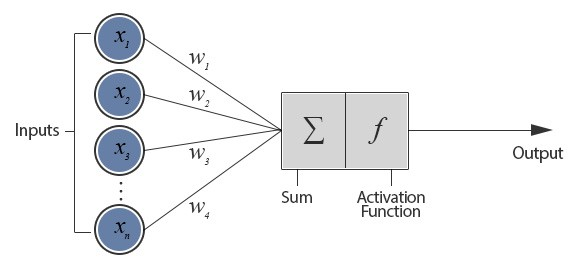
\includegraphics[width=0.8\textwidth]{neuron.jpeg}
\caption{Model of an artificial neuron.}
\end{figure}

A neuron (or more generally a perceptron) consists of weights (\(w_i\))
and real (\(x_i\)) numbers. All the inputs are individually weighted,
added together and passed into the activation function. There are many
different types of activation function but one of the simplest would be
step function (another is the sigmoid).

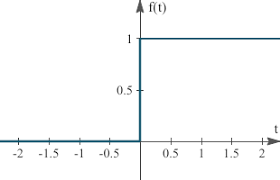
\includegraphics[width=0.45\textwidth]{step_function.png} 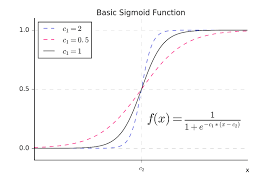
\includegraphics[width=0.45\textwidth]{sigmoid.png}

\hypertarget{training-of-perceptrons}{%
\subsubsection{Training of perceptrons}\label{training-of-perceptrons}}

When teaching children how to recognize a bus, we just tell them,
showing an example: ``This is a bus. That is not a bus.'' until they
learn the concept of what a bus is. Furthermore, if the child sees new
objects that she hasn't seen before, we could expect her to recognize
correctly whether the new object is a bus or not. This is exactly the
idea behind the perceptron. Similarly, inputs from a \emph{training} set
are presented to the perceptron one after the other and weights are
modified according to the expected output.

When an entire pass through all of the input training vectors is
completed the perceptron has learnt ! At this time, if an input vector P
(already in the training set) is given to the perceptron, it will output
the correct value. If P is not in the training set, the network will
respond with an output similar to other training vectors close to P.

Unfortunately using just a perceptron is not too useful since it is not
possible to solve the interesting problems we would like to face. The
next step is then to put together more perceptron together in
\emph{layers}.

\hypertarget{multi-layered-neural-networks}{%
\subsubsection{Multi-layered neural
networks}\label{multi-layered-neural-networks}}

\begin{figure}
\centering
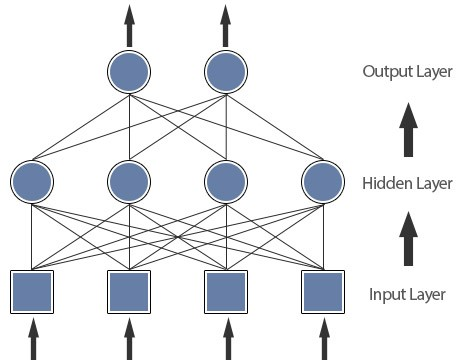
\includegraphics[width=0.8\textwidth]{multilayer.jpeg}
\caption{A multi-layered neural network.}
\end{figure}

Each input from the \emph{input layer} is fed up to each node in the
hidden layer, and from there to each node on the output layer. We should
note that there can be any number of nodes per layer and there are
usually multiple hidden layers to pass through before ultimately
reaching the output layer. But to train this network we need a learning
algorithm which should be able to tune not only the weights between the
output layer and the hidden layer but also the weights between the
hidden layer and the input layer.

\hypertarget{back-propagation}{%
\subsubsection{Back propagation}\label{back-propagation}}

First of all, we need to understand what do we lack. To tune the weights
between the hidden layer and the input layer, we need to know the error
at the hidden layer, but we know the error only at the output layer (We
know the correct output from the training sample and we also know the
output predicted by the network.) So, the method that was suggested was
to take the errors at the output layer and proportionally propagate them
backwards to the hidden layer.

So, what we are doing is:

\begin{itemize}
\tightlist
\item
  We present a training sample to the neural network (initialised with
  random weights)
\item
  Compute the output received by calculating activations of each layer
  and thus calculate the error
\item
  Having calculated the error, we readjust the weights such that the
  error decreases
\item
  We continue the process for all training samples several times until
  the weights are not changing too much
\end{itemize}

\hypertarget{neural-net-to-recognize-handwritten-digits}{%
\subsection{Neural net to recognize handwritten
digits}\label{neural-net-to-recognize-handwritten-digits}}

We don't usually appreciate how tough a problem our visual system solve
(it involves 5 visual cortices containing 140 million neurons each). The
difficulty of visual pattern recognition becomes apparent if you attempt
to write a computer program to recognize digits like those below.

\begin{figure}
\centering
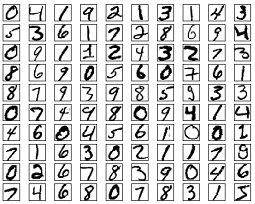
\includegraphics{mnist_100_digits.png}
\caption{The so-called MNIST training sample}
\end{figure}

Simple intuitions about how we recognize shapes - ``a 9 has a loop at
the top, and a vertical stroke in the bottom right'' - turn out to be
not so simple to express algorithmically. When you try to make such
rules precise, you quickly get lost in a morass of exceptions and
caveats and special cases. It seems hopeless.

Neural networks approach the problem in a different way. The idea is to
take a large number of handwritten digits and then develop a system
which can learn from those training examples. By increasing the number
of training examples, the network can learn more about handwriting, and
so improve its accuracy. So while I've shown just 100 training digits
above, perhaps we could build a better handwriting recognizer by using
thousands or even millions or billions of training examples
(\textbf{remember that neural nets are not capable of extrapolating
results !!!}).

Let's try to implement an ANN that is capable of recognize handwritten
digits. To start we need to install two new modules (from the command
line type the following):

\texttt{pip\ install\ keras,\ mnist,\ tensorflow}

Our program will be based on a Convolutional Neural Network (CNN, will
see later other two types of NN) which is designed for image/pattern
recognition. It works essentially by applying on top of an image a
series of filters (matrices) that works as edge detectors and with them
it classifies images according to their features.

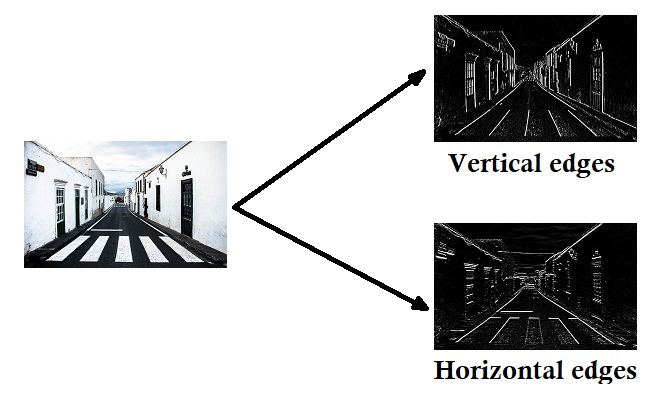
\includegraphics[width=0.8\textwidth]{edges.jpg}

    \begin{Verbatim}[commandchars=\\\{\}]
{\color{incolor}In [{\color{incolor}2}]:} \PY{k+kn}{import} \PY{n+nn}{numpy} \PY{k}{as} \PY{n+nn}{np}
        \PY{c+c1}{\PYZsh{} contains our dataset for training}
        \PY{k+kn}{import} \PY{n+nn}{mnist} 
        \PY{c+c1}{\PYZsh{} keras gives us all the tools to work with NN}
        \PY{k+kn}{from} \PY{n+nn}{keras}\PY{n+nn}{.}\PY{n+nn}{models} \PY{k}{import} \PY{n}{Sequential} 
        \PY{k+kn}{from} \PY{n+nn}{keras}\PY{n+nn}{.}\PY{n+nn}{layers} \PY{k}{import} \PY{n}{Conv2D}\PY{p}{,} \PY{n}{MaxPooling2D}\PY{p}{,} \PY{n}{Dense}\PY{p}{,} \PY{n}{Flatten}
        \PY{k+kn}{from} \PY{n+nn}{keras}\PY{n+nn}{.}\PY{n+nn}{utils} \PY{k}{import} \PY{n}{to\PYZus{}categorical}
        
        \PY{c+c1}{\PYZsh{} load the training and testing set}
        \PY{n}{train\PYZus{}images} \PY{o}{=} \PY{n}{mnist}\PY{o}{.}\PY{n}{train\PYZus{}images}\PY{p}{(}\PY{p}{)} \PY{c+c1}{\PYZsh{} the actual images}
        \PY{n}{train\PYZus{}labels} \PY{o}{=} \PY{n}{mnist}\PY{o}{.}\PY{n}{train\PYZus{}labels}\PY{p}{(}\PY{p}{)} \PY{c+c1}{\PYZsh{} the truth (it is 0, 1, 2...)}
        \PY{n}{test\PYZus{}images} \PY{o}{=} \PY{n}{mnist}\PY{o}{.}\PY{n}{test\PYZus{}images}\PY{p}{(}\PY{p}{)}
        \PY{n}{test\PYZus{}labels} \PY{o}{=} \PY{n}{mnist}\PY{o}{.}\PY{n}{test\PYZus{}labels}\PY{p}{(}\PY{p}{)}
        
        \PY{c+c1}{\PYZsh{} transform data for convenience}
        \PY{n}{train\PYZus{}images} \PY{o}{=} \PY{p}{(}\PY{n}{train\PYZus{}images} \PY{o}{/} \PY{l+m+mi}{255}\PY{p}{)} \PY{o}{\PYZhy{}} \PY{l+m+mf}{0.5}
        \PY{n}{test\PYZus{}images} \PY{o}{=} \PY{p}{(}\PY{n}{test\PYZus{}images} \PY{o}{/} \PY{l+m+mi}{255}\PY{p}{)} \PY{o}{\PYZhy{}} \PY{l+m+mf}{0.5}
        \PY{n}{train\PYZus{}images} \PY{o}{=} \PY{n}{np}\PY{o}{.}\PY{n}{expand\PYZus{}dims}\PY{p}{(}\PY{n}{train\PYZus{}images}\PY{p}{,} \PY{n}{axis}\PY{o}{=}\PY{l+m+mi}{3}\PY{p}{)}
        \PY{n}{test\PYZus{}images} \PY{o}{=} \PY{n}{np}\PY{o}{.}\PY{n}{expand\PYZus{}dims}\PY{p}{(}\PY{n}{test\PYZus{}images}\PY{p}{,} \PY{n}{axis}\PY{o}{=}\PY{l+m+mi}{3}\PY{p}{)}
        
        \PY{c+c1}{\PYZsh{} definition of the actual network}
        \PY{n}{num\PYZus{}filters} \PY{o}{=} \PY{l+m+mi}{8}
        \PY{n}{filter\PYZus{}size} \PY{o}{=} \PY{l+m+mi}{3}
        \PY{n}{pool\PYZus{}size} \PY{o}{=} \PY{l+m+mi}{2}
        
        \PY{c+c1}{\PYZsh{} the input size reflects the size of the image with}
        \PY{c+c1}{\PYZsh{} the numbers 28x28 pixels}
        \PY{c+c1}{\PYZsh{} the output is given by 10 neurons returning the }
        \PY{c+c1}{\PYZsh{} probability that image is in each class.}
        \PY{n}{model} \PY{o}{=} \PY{n}{Sequential}\PY{p}{(}\PY{p}{[}
            \PY{n}{Conv2D}\PY{p}{(}\PY{n}{num\PYZus{}filters}\PY{p}{,} \PY{n}{filter\PYZus{}size}\PY{p}{,} \PY{n}{input\PYZus{}shape}\PY{o}{=}\PY{p}{(}\PY{l+m+mi}{28}\PY{p}{,} \PY{l+m+mi}{28}\PY{p}{,} \PY{l+m+mi}{1}\PY{p}{)}\PY{p}{)}\PY{p}{,} 
            \PY{n}{MaxPooling2D}\PY{p}{(}\PY{n}{pool\PYZus{}size}\PY{o}{=}\PY{n}{pool\PYZus{}size}\PY{p}{)}\PY{p}{,}
            \PY{n}{Flatten}\PY{p}{(}\PY{p}{)}\PY{p}{,}
            \PY{n}{Dense}\PY{p}{(}\PY{l+m+mi}{10}\PY{p}{,} \PY{n}{activation}\PY{o}{=}\PY{l+s+s2}{\PYZdq{}}\PY{l+s+s2}{softmax}\PY{l+s+s2}{\PYZdq{}}\PY{p}{)}
        \PY{p}{]}\PY{p}{)}
        
        \PY{n}{model}\PY{o}{.}\PY{n}{compile}\PY{p}{(}\PY{l+s+s1}{\PYZsq{}}\PY{l+s+s1}{adam}\PY{l+s+s1}{\PYZsq{}}\PY{p}{,} \PY{n}{loss}\PY{o}{=}\PY{l+s+s2}{\PYZdq{}}\PY{l+s+s2}{categorical\PYZus{}crossentropy}\PY{l+s+s2}{\PYZdq{}}\PY{p}{,}
                      \PY{n}{metrics}\PY{o}{=}\PY{p}{[}\PY{l+s+s1}{\PYZsq{}}\PY{l+s+s1}{accuracy}\PY{l+s+s1}{\PYZsq{}}\PY{p}{]}\PY{p}{)}
        
        \PY{n}{model}\PY{o}{.}\PY{n}{fit}\PY{p}{(}\PY{n}{train\PYZus{}images}\PY{p}{,}
                  \PY{n}{to\PYZus{}categorical}\PY{p}{(}\PY{n}{train\PYZus{}labels}\PY{p}{)}\PY{p}{,}
                  \PY{n}{epochs}\PY{o}{=}\PY{l+m+mi}{3}\PY{p}{,}
                  \PY{n}{validation\PYZus{}data}\PY{o}{=}\PY{p}{(}\PY{n}{test\PYZus{}images}\PY{p}{,} \PY{n}{to\PYZus{}categorical}\PY{p}{(}\PY{n}{test\PYZus{}labels}\PY{p}{)}\PY{p}{)}\PY{p}{)}
\end{Verbatim}

    \begin{Verbatim}[commandchars=\\\{\}]
Using TensorFlow backend.

    \end{Verbatim}

    \begin{Verbatim}[commandchars=\\\{\}]
Train on 60000 samples, validate on 10000 samples
Epoch 1/3
60000/60000 [==============================] - 13s 222us/step - loss: 0.3369 - acc: 0.9025 - val\_loss: 0.1855 - val\_acc: 0.9461
Epoch 2/3
60000/60000 [==============================] - 14s 228us/step - loss: 0.1633 - acc: 0.9531 - val\_loss: 0.1273 - val\_acc: 0.9630
Epoch 3/3
60000/60000 [==============================] - 14s 226us/step - loss: 0.1211 - acc: 0.9649 - val\_loss: 0.1092 - val\_acc: 0.9682

    \end{Verbatim}

\begin{Verbatim}[commandchars=\\\{\}]
{\color{outcolor}Out[{\color{outcolor}2}]:} <keras.callbacks.History at 0x7f3bd6db5390>
\end{Verbatim}
            
    \begin{Verbatim}[commandchars=\\\{\}]
{\color{incolor}In [{\color{incolor}10}]:} \PY{n}{predictions} \PY{o}{=} \PY{n}{model}\PY{o}{.}\PY{n}{predict}\PY{p}{(}\PY{n}{test\PYZus{}images}\PY{p}{[}\PY{l+m+mi}{0}\PY{p}{:}\PY{l+m+mi}{2}\PY{p}{]}\PY{p}{)}
         \PY{k}{for} \PY{n}{p} \PY{o+ow}{in} \PY{n}{predictions}\PY{p}{:}
             \PY{n+nb}{print} \PY{p}{(}\PY{p}{[}\PY{l+s+s2}{\PYZdq{}}\PY{l+s+si}{\PYZob{}:.2f\PYZcb{}}\PY{l+s+s2}{\PYZdq{}}\PY{o}{.}\PY{n}{format}\PY{p}{(}\PY{n}{i}\PY{p}{)} \PY{k}{for} \PY{n}{i} \PY{o+ow}{in} \PY{n}{p}\PY{p}{]}\PY{p}{)}
         
         \PY{k}{for} \PY{n}{i} \PY{o+ow}{in} \PY{n+nb}{range}\PY{p}{(}\PY{l+m+mi}{2}\PY{p}{)}\PY{p}{:}
             \PY{n+nb}{print}\PY{p}{(}\PY{l+s+s2}{\PYZdq{}}\PY{l+s+s2}{The CNN predicted }\PY{l+s+si}{\PYZob{}\PYZcb{}}\PY{l+s+s2}{ and it was }\PY{l+s+si}{\PYZob{}\PYZcb{}}\PY{l+s+s2}{\PYZdq{}}\PY{o}{.}\PY{n}{format}\PY{p}{(} \PYZbs{}
                   \PY{n}{np}\PY{o}{.}\PY{n}{argmax}\PY{p}{(}\PY{n}{predictions}\PY{p}{[}\PY{n}{i}\PY{p}{]}\PY{p}{,} \PY{n}{axis}\PY{o}{=}\PY{l+m+mi}{0}\PY{p}{)}\PY{p}{,} \PY{n}{test\PYZus{}labels}\PY{p}{[}\PY{n}{i}\PY{p}{]}\PY{p}{)}\PY{p}{)}
\end{Verbatim}

    \begin{Verbatim}[commandchars=\\\{\}]
['0.00', '0.00', '0.00', '0.00', '0.00', '0.00', '0.00', '1.00', '0.00', '0.00']
['0.00', '0.00', '0.99', '0.00', '0.00', '0.00', '0.01', '0.00', '0.00', '0.00']
The CNN predicted 7 and it was 7
The CNN predicted 2 and it was 2

    \end{Verbatim}

    I have tested the NN using digits written by me:
    
    \begin{center}
      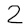
\includegraphics[width=0.3\textwidth]{due.png}
      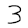
\includegraphics[width=0.3\textwidth]{tre.png}
      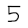
\includegraphics[width=0.3\textwidth]{cinque.png}
    \end{center}
    
and the ANN worked with the three of them. This is the result with my 5:

\begin{Shaded}
\begin{Highlighting}[]
\NormalTok{[}\DecValTok{5}\NormalTok{]}
\NormalTok{[}\FloatTok{0.00}\NormalTok{, }\FloatTok{0.00}\NormalTok{, }\FloatTok{0.00}\NormalTok{, }\FloatTok{0.10}\NormalTok{, }\FloatTok{0.00}\NormalTok{, }\FloatTok{0.89}\NormalTok{, }\FloatTok{0.00}\NormalTok{, }\FloatTok{0.00}\NormalTok{, }\FloatTok{0.00}\NormalTok{, }\FloatTok{0.00}\NormalTok{]}
\end{Highlighting}
\end{Shaded}

Smaller probability \emph{only} 89.4\% (confused by the 3 10\%) \textbf{but
still it works}.

\hypertarget{black-scholes-call-options}{%
\subsection{Black-Scholes call
options}\label{black-scholes-call-options}}

The first practical application concerns the pricing of european call
options. In this case I have generated by myself a large number of call
options with different strikes, maturity, underlying development and
trained the NN using as inputs: volatility, strike, maturity and
underlying price. The truth is the price of the call computed using the
Black-Scholes formula.


\includegraphics[width=0.7\textwidth]{underlyings.png}

In this case I have used a \emph{traditional} NN with an input layer
with 5 neurons (the number of inputs), an hidden layer with 8 neurons
and an output layer with 1 single neuron (since I need just a number,
the price of the call).

    \begin{Verbatim}[commandchars=\\\{\}]
{\color{incolor}In [{\color{incolor} }]:} \PY{c+c1}{\PYZsh{} Regression Example }
        \PY{k+kn}{from} \PY{n+nn}{keras}\PY{n+nn}{.}\PY{n+nn}{models} \PY{k}{import} \PY{n}{Sequential}\PY{p}{,} \PY{n}{load\PYZus{}model}
        \PY{k+kn}{from} \PY{n+nn}{keras}\PY{n+nn}{.}\PY{n+nn}{layers} \PY{k}{import} \PY{n}{Dense}
        \PY{k+kn}{from} \PY{n+nn}{keras}\PY{n+nn}{.}\PY{n+nn}{optimizers} \PY{k}{import} \PY{n}{SGD}
        \PY{k+kn}{from} \PY{n+nn}{keras}\PY{n+nn}{.}\PY{n+nn}{wrappers}\PY{n+nn}{.}\PY{n+nn}{scikit\PYZus{}learn} \PY{k}{import} \PY{n}{KerasRegressor}
        \PY{k+kn}{from} \PY{n+nn}{sklearn}\PY{n+nn}{.}\PY{n+nn}{model\PYZus{}selection} \PY{k}{import} \PY{n}{cross\PYZus{}val\PYZus{}score}
        \PY{k+kn}{from} \PY{n+nn}{sklearn}\PY{n+nn}{.}\PY{n+nn}{model\PYZus{}selection} \PY{k}{import} \PY{n}{train\PYZus{}test\PYZus{}split}
        \PY{k+kn}{from} \PY{n+nn}{sklearn}\PY{n+nn}{.}\PY{n+nn}{metrics} \PY{k}{import} \PY{n}{accuracy\PYZus{}score}
        \PY{k+kn}{import} \PY{n+nn}{pandas} \PY{k}{as} \PY{n+nn}{pd}
        \PY{k+kn}{import} \PY{n+nn}{matplotlib}\PY{n+nn}{.}\PY{n+nn}{pyplot} \PY{k}{as} \PY{n+nn}{plt}
        
        \PY{c+c1}{\PYZsh{}\PYZsh{} just a way to load the dataset}
        \PY{n}{dataset} \PY{o}{=} \PY{n}{pd}\PY{o}{.}\PY{n}{read\PYZus{}csv}\PY{p}{(}\PY{l+s+s2}{\PYZdq{}}\PY{l+s+s2}{training.csv}\PY{l+s+s2}{\PYZdq{}}\PY{p}{)}
        \PY{n}{X\PYZus{}train} \PY{o}{=} \PY{n}{dataset}\PY{o}{.}\PY{n}{iloc}\PY{p}{[}\PY{p}{:}\PY{p}{,} \PY{p}{:}\PY{l+m+mi}{5}\PY{p}{]}\PY{o}{.}\PY{n}{values}
        \PY{n}{Y\PYZus{}train} \PY{o}{=} \PY{n}{dataset}\PY{o}{.}\PY{n}{iloc}\PY{p}{[}\PY{p}{:}\PY{p}{,} \PY{l+m+mi}{5}\PY{p}{]}\PY{o}{.}\PY{n}{values}
        
        \PY{c+c1}{\PYZsh{} NN defintion}
        \PY{n}{model} \PY{o}{=} \PY{n}{Sequential}\PY{p}{(}\PY{p}{)}
        \PY{n}{model}\PY{o}{.}\PY{n}{add}\PY{p}{(}\PY{n}{Dense}\PY{p}{(}\PY{l+m+mi}{8}\PY{p}{,} \PY{n}{input\PYZus{}dim}\PY{o}{=}\PY{l+m+mi}{5}\PY{p}{,} 
                        \PY{n}{kernel\PYZus{}initializer}\PY{o}{=}\PY{l+s+s1}{\PYZsq{}}\PY{l+s+s1}{normal}\PY{l+s+s1}{\PYZsq{}}\PY{p}{,} 
                        \PY{n}{activation}\PY{o}{=}\PY{l+s+s1}{\PYZsq{}}\PY{l+s+s1}{relu}\PY{l+s+s1}{\PYZsq{}}\PY{p}{)}\PY{p}{)}
        \PY{n}{model}\PY{o}{.}\PY{n}{add}\PY{p}{(}\PY{n}{Dense}\PY{p}{(}\PY{l+m+mi}{11}\PY{p}{,} \PY{n}{kernel\PYZus{}initializer}\PY{o}{=}\PY{l+s+s1}{\PYZsq{}}\PY{l+s+s1}{normal}\PY{l+s+s1}{\PYZsq{}}\PY{p}{,} 
                        \PY{n}{activation}\PY{o}{=}\PY{l+s+s1}{\PYZsq{}}\PY{l+s+s1}{relu}\PY{l+s+s1}{\PYZsq{}}\PY{p}{)}\PY{p}{)}
        \PY{n}{model}\PY{o}{.}\PY{n}{add}\PY{p}{(}\PY{n}{Dense}\PY{p}{(}\PY{l+m+mi}{1}\PY{p}{,} \PY{n}{kernel\PYZus{}initializer}\PY{o}{=}\PY{l+s+s1}{\PYZsq{}}\PY{l+s+s1}{normal}\PY{l+s+s1}{\PYZsq{}}\PY{p}{)}\PY{p}{)}
        
        \PY{c+c1}{\PYZsh{} Compile model}
        \PY{n}{model}\PY{o}{.}\PY{n}{compile}\PY{p}{(}\PY{n}{loss}\PY{o}{=}\PY{l+s+s1}{\PYZsq{}}\PY{l+s+s1}{mean\PYZus{}absolute\PYZus{}error}\PY{l+s+s1}{\PYZsq{}}\PY{p}{,} 
                      \PY{n}{optimizer}\PY{o}{=}\PY{l+s+s1}{\PYZsq{}}\PY{l+s+s1}{adam}\PY{l+s+s1}{\PYZsq{}}\PY{p}{,} 
                      \PY{n}{metrics}\PY{o}{=}\PY{p}{[}\PY{l+s+s1}{\PYZsq{}}\PY{l+s+s1}{mse}\PY{l+s+s1}{\PYZsq{}}\PY{p}{]}\PY{p}{)}
        
        \PY{c+c1}{\PYZsh{} perform the actual training}
        \PY{n}{history} \PY{o}{=} \PY{n}{model}\PY{o}{.}\PY{n}{fit}\PY{p}{(}\PY{n}{X\PYZus{}train}\PY{p}{,} 
                            \PY{n}{Y\PYZus{}train}\PY{p}{,} 
                            \PY{n}{epochs}\PY{o}{=}\PY{l+m+mi}{100}\PY{p}{,} 
                            \PY{n}{verbose}\PY{o}{=}\PY{l+m+mi}{1}\PY{p}{,} 
                            \PY{n}{batch\PYZus{}size}\PY{o}{=}\PY{l+m+mi}{100}\PY{p}{)}
\end{Verbatim}

    The training of a neural net is stochastic so it should be run multiple
times to asses its performance.

    \begin{Verbatim}[commandchars=\\\{\}]
{\color{incolor}In [{\color{incolor}13}]:} \PY{k+kn}{import} \PY{n+nn}{pandas} \PY{k}{as} \PY{n+nn}{pd}
         \PY{k+kn}{from} \PY{n+nn}{keras}\PY{n+nn}{.}\PY{n+nn}{models} \PY{k}{import} \PY{n}{load\PYZus{}model}
         \PY{k+kn}{import} \PY{n+nn}{matplotlib}\PY{n+nn}{.}\PY{n+nn}{pyplot} \PY{k}{as} \PY{n+nn}{plt}
         
         \PY{n}{model} \PY{o}{=} \PY{n}{load\PYZus{}model}\PY{p}{(}\PY{l+s+s1}{\PYZsq{}}\PY{l+s+s1}{bs\PYZus{}model.h5.very\PYZus{}very\PYZus{}good}\PY{l+s+s1}{\PYZsq{}}\PY{p}{)}
         
         \PY{n}{dataset} \PY{o}{=} \PY{n}{pd}\PY{o}{.}\PY{n}{read\PYZus{}csv}\PY{p}{(}\PY{l+s+s2}{\PYZdq{}}\PY{l+s+s2}{testing.csv}\PY{l+s+s2}{\PYZdq{}}\PY{p}{)}
         \PY{n}{X\PYZus{}test} \PY{o}{=} \PY{n}{dataset}\PY{o}{.}\PY{n}{iloc}\PY{p}{[}\PY{p}{:}\PY{p}{,} \PY{p}{:}\PY{l+m+mi}{5}\PY{p}{]}\PY{o}{.}\PY{n}{values}
         \PY{n}{Y\PYZus{}test} \PY{o}{=} \PY{n}{dataset}\PY{o}{.}\PY{n}{iloc}\PY{p}{[}\PY{p}{:}\PY{p}{,} \PY{l+m+mi}{5}\PY{p}{]}\PY{o}{.}\PY{n}{values}
         
         \PY{n}{plt}\PY{o}{.}\PY{n}{plot}\PY{p}{(}\PY{n}{model}\PY{o}{.}\PY{n}{predict}\PY{p}{(}\PY{n}{X\PYZus{}test}\PY{p}{[}\PY{l+m+mi}{0}\PY{p}{:}\PY{l+m+mi}{200}\PY{p}{]}\PY{p}{)}\PY{p}{)}
         \PY{n}{plt}\PY{o}{.}\PY{n}{plot}\PY{p}{(}\PY{n}{Y\PYZus{}test}\PY{p}{[}\PY{l+m+mi}{0}\PY{p}{:}\PY{l+m+mi}{200}\PY{p}{]}\PY{p}{)}
         \PY{n}{plt}\PY{o}{.}\PY{n}{show}\PY{p}{(}\PY{p}{)}
\end{Verbatim}

    \begin{center}
    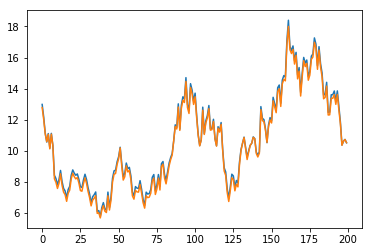
\includegraphics[width=0.7\textwidth]{lecture_10_6_0.png}
    \end{center}
    { \hspace*{\fill} \\}
    
    \hypertarget{technical-analysis}{%
\subsection{Technical Analysis}\label{technical-analysis}}

In finance, technical analysis is a security analysis discipline for
forecasting the direction of prices through the study of past market
data, primarily price and volume. Essentially the analyst looks for
particular patterns in the price time series that are \emph{known} to
develop in predictable ways to take profit of it.

\begin{center}
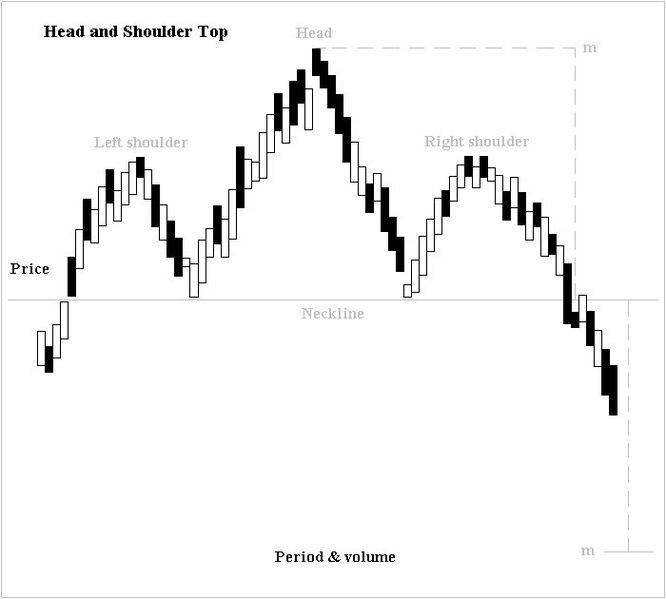
\includegraphics[width=0.6\textwidth]{H_and_s_top_new.jpg}
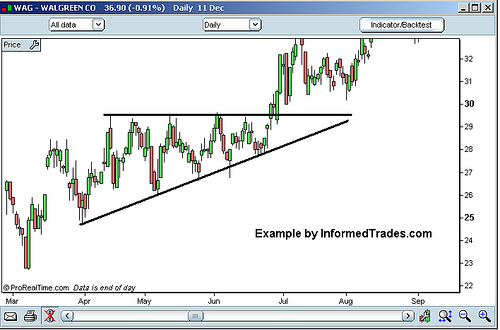
\includegraphics[width=0.6\textwidth]{Triangle-ascending.jpg}
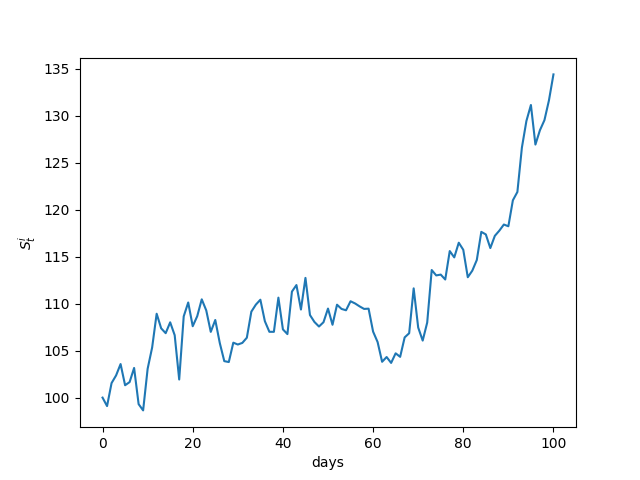
\includegraphics[width=0.6\textwidth]{image_1.png}
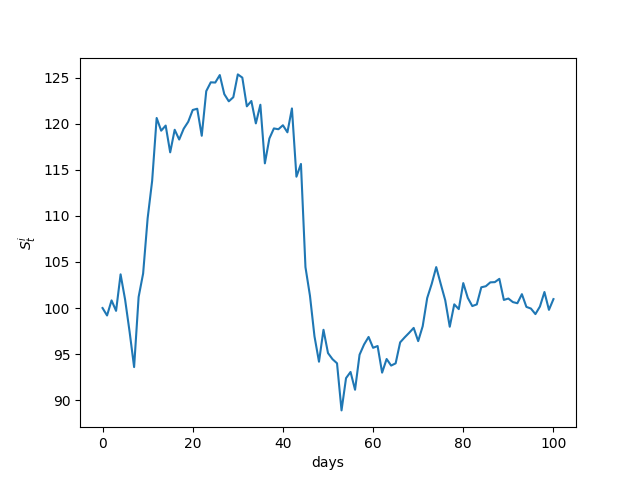
\includegraphics[width=0.6\textwidth]{image_2.png}
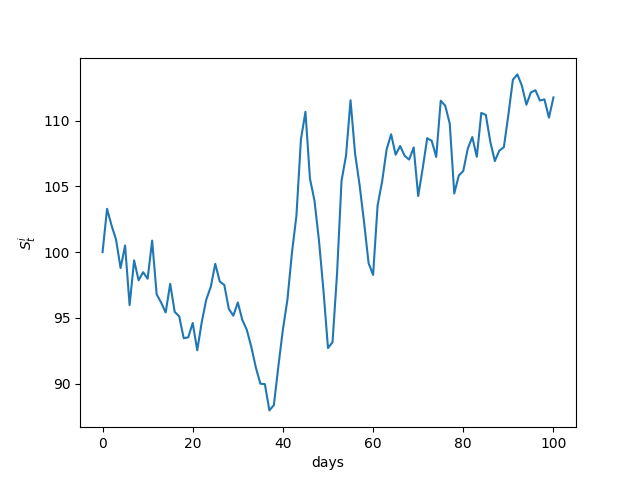
\includegraphics[width=0.6\textwidth]{image_0.png}
\end{center}

As you may imagine we will try to develop a CNN (like in the handwriting
case) capable of classifying features in time series to be used in a
technical analysis (this is much faster than having somebody looking at
thousands of time series by eye\ldots{}).

As in the previous application I have generated by myself the training
set simulating 9000 time series (1/3 with head and shoulder patter, 1/3
with triangle pattern and 1/3 with no pattern). To make the training
easier the features have been exagerated.

No pattern

Head and shoulder pattern

Tringle pattern

    \begin{Verbatim}[commandchars=\\\{\}]
{\color{incolor}In [{\color{incolor}17}]:} \PY{k+kn}{import} \PY{n+nn}{numpy} \PY{k}{as} \PY{n+nn}{np}
         \PY{k+kn}{import} \PY{n+nn}{json}
         \PY{k+kn}{from} \PY{n+nn}{keras}\PY{n+nn}{.}\PY{n+nn}{models} \PY{k}{import} \PY{n}{Sequential}\PY{p}{,} \PY{n}{load\PYZus{}model}
         \PY{k+kn}{from} \PY{n+nn}{keras}\PY{n+nn}{.}\PY{n+nn}{layers} \PY{k}{import} \PY{n}{Dense}\PY{p}{,} \PY{n}{Conv1D}\PY{p}{,} \PY{n}{Dropout}
         \PY{k+kn}{from} \PY{n+nn}{keras}\PY{n+nn}{.}\PY{n+nn}{layers} \PY{k}{import} \PY{n}{MaxPooling1D}\PY{p}{,} \PY{n}{GlobalAveragePooling1D}
         \PY{k+kn}{from} \PY{n+nn}{keras}\PY{n+nn}{.}\PY{n+nn}{utils} \PY{k}{import} \PY{n}{to\PYZus{}categorical}
         
         \PY{c+c1}{\PYZsh{} load the training set}
         \PY{k}{with} \PY{n+nb}{open}\PY{p}{(}\PY{l+s+s2}{\PYZdq{}}\PY{l+s+s2}{training\PYZus{}tech\PYZus{}ana\PYZus{}labels.json}\PY{l+s+s2}{\PYZdq{}}\PY{p}{,} \PY{l+s+s2}{\PYZdq{}}\PY{l+s+s2}{r}\PY{l+s+s2}{\PYZdq{}}\PY{p}{)} \PY{k}{as} \PY{n}{f}\PY{p}{:}
             \PY{n}{train\PYZus{}labels} \PY{o}{=} \PY{n}{json}\PY{o}{.}\PY{n}{load}\PY{p}{(}\PY{n}{f}\PY{p}{)}
         
         \PY{n}{train\PYZus{}labels} \PY{o}{=} \PY{n}{train\PYZus{}labels}\PY{p}{[}\PY{p}{:}\PY{l+m+mi}{900}\PY{p}{]}
         \PY{n}{train\PYZus{}images} \PY{o}{=} \PY{p}{[}\PY{p}{]}
         
         \PY{k}{with} \PY{n+nb}{open}\PY{p}{(}\PY{l+s+s2}{\PYZdq{}}\PY{l+s+s2}{training\PYZus{}tech\PYZus{}ana\PYZus{}images.json}\PY{l+s+s2}{\PYZdq{}}\PY{p}{,} \PY{l+s+s2}{\PYZdq{}}\PY{l+s+s2}{r}\PY{l+s+s2}{\PYZdq{}}\PY{p}{)} \PY{k}{as} \PY{n}{f}\PY{p}{:}
             \PY{n}{train\PYZus{}images} \PY{o}{=} \PY{n}{json}\PY{o}{.}\PY{n}{load}\PY{p}{(}\PY{n}{f}\PY{p}{)}
         \PY{n}{train\PYZus{}images} \PY{o}{=} \PY{n}{train\PYZus{}images}\PY{p}{[}\PY{p}{:}\PY{l+m+mi}{900}\PY{p}{]}
         
         \PY{n}{train\PYZus{}images} \PY{o}{=} \PY{n}{np}\PY{o}{.}\PY{n}{array}\PY{p}{(}\PY{n}{train\PYZus{}images}\PY{p}{)}
         \PY{n}{train\PYZus{}images} \PY{o}{=} \PY{n}{np}\PY{o}{.}\PY{n}{expand\PYZus{}dims}\PY{p}{(}\PY{n}{train\PYZus{}images}\PY{p}{,} \PY{n}{axis}\PY{o}{=}\PY{l+m+mi}{3}\PY{p}{)}
         
         \PY{c+c1}{\PYZsh{} define the CNN }
         \PY{n}{model} \PY{o}{=} \PY{n}{Sequential}\PY{p}{(}\PY{p}{)}
         \PY{n}{model}\PY{o}{.}\PY{n}{add}\PY{p}{(}\PY{n}{Conv1D}\PY{p}{(}\PY{n}{filters}\PY{o}{=}\PY{l+m+mi}{80}\PY{p}{,} \PY{n}{kernel\PYZus{}size}\PY{o}{=}\PY{l+m+mi}{20}\PY{p}{,} 
                          \PY{n}{activation}\PY{o}{=}\PY{l+s+s1}{\PYZsq{}}\PY{l+s+s1}{relu}\PY{l+s+s1}{\PYZsq{}}\PY{p}{,} \PY{n}{input\PYZus{}shape}\PY{o}{=}\PY{p}{(}\PY{l+m+mi}{101}\PY{p}{,} \PY{l+m+mi}{1}\PY{p}{)}\PY{p}{)}\PY{p}{)}
         \PY{n}{model}\PY{o}{.}\PY{n}{add}\PY{p}{(}\PY{n}{Conv1D}\PY{p}{(}\PY{n}{filters}\PY{o}{=}\PY{l+m+mi}{80}\PY{p}{,} \PY{n}{kernel\PYZus{}size}\PY{o}{=}\PY{l+m+mi}{15}\PY{p}{,} 
                          \PY{n}{activation}\PY{o}{=}\PY{l+s+s1}{\PYZsq{}}\PY{l+s+s1}{relu}\PY{l+s+s1}{\PYZsq{}}\PY{p}{)}\PY{p}{)}
         \PY{n}{model}\PY{o}{.}\PY{n}{add}\PY{p}{(}\PY{n}{MaxPooling1D}\PY{p}{(}\PY{l+m+mi}{3}\PY{p}{)}\PY{p}{)}
         \PY{n}{model}\PY{o}{.}\PY{n}{add}\PY{p}{(}\PY{n}{Conv1D}\PY{p}{(}\PY{n}{filters}\PY{o}{=}\PY{l+m+mi}{100}\PY{p}{,} \PY{n}{kernel\PYZus{}size}\PY{o}{=}\PY{l+m+mi}{10}\PY{p}{,} 
                          \PY{n}{activation}\PY{o}{=}\PY{l+s+s1}{\PYZsq{}}\PY{l+s+s1}{relu}\PY{l+s+s1}{\PYZsq{}}\PY{p}{)}\PY{p}{)}
         \PY{n}{model}\PY{o}{.}\PY{n}{add}\PY{p}{(}\PY{n}{Conv1D}\PY{p}{(}\PY{n}{filters}\PY{o}{=}\PY{l+m+mi}{100}\PY{p}{,} \PY{n}{kernel\PYZus{}size}\PY{o}{=}\PY{l+m+mi}{5}\PY{p}{,} 
                          \PY{n}{activation}\PY{o}{=}\PY{l+s+s1}{\PYZsq{}}\PY{l+s+s1}{relu}\PY{l+s+s1}{\PYZsq{}}\PY{p}{)}\PY{p}{)}
         \PY{n}{model}\PY{o}{.}\PY{n}{add}\PY{p}{(}\PY{n}{GlobalAveragePooling1D}\PY{p}{(}\PY{p}{)}\PY{p}{)}
         \PY{n}{model}\PY{o}{.}\PY{n}{add}\PY{p}{(}\PY{n}{Dropout}\PY{p}{(}\PY{l+m+mf}{0.5}\PY{p}{)}\PY{p}{)}
         \PY{n}{model}\PY{o}{.}\PY{n}{add}\PY{p}{(}\PY{n}{Dense}\PY{p}{(}\PY{l+m+mi}{3}\PY{p}{,} \PY{n}{activation}\PY{o}{=}\PY{l+s+s2}{\PYZdq{}}\PY{l+s+s2}{softmax}\PY{l+s+s2}{\PYZdq{}}\PY{p}{)}\PY{p}{)}
         \PY{n}{model}\PY{o}{.}\PY{n}{compile}\PY{p}{(}\PY{n}{loss}\PY{o}{=}\PY{l+s+s1}{\PYZsq{}}\PY{l+s+s1}{categorical\PYZus{}crossentropy}\PY{l+s+s1}{\PYZsq{}}\PY{p}{,} 
                       \PY{n}{optimizer}\PY{o}{=}\PY{l+s+s1}{\PYZsq{}}\PY{l+s+s1}{adam}\PY{l+s+s1}{\PYZsq{}}\PY{p}{,} \PY{n}{metrics}\PY{o}{=}\PY{p}{[}\PY{l+s+s1}{\PYZsq{}}\PY{l+s+s1}{accuracy}\PY{l+s+s1}{\PYZsq{}}\PY{p}{]}\PY{p}{)}
         
         \PY{c+c1}{\PYZsh{} make the training}
         \PY{n}{model}\PY{o}{.}\PY{n}{fit}\PY{p}{(}\PY{n}{train\PYZus{}images}\PY{p}{,} \PY{n}{to\PYZus{}categorical}\PY{p}{(}\PY{n}{train\PYZus{}labels}\PY{p}{)}\PY{p}{,} 
                   \PY{n}{epochs}\PY{o}{=}\PY{l+m+mi}{150}\PY{p}{,} \PY{n}{batch\PYZus{}size}\PY{o}{=}\PY{l+m+mi}{35}\PY{p}{,} \PY{n}{verbose}\PY{o}{=}\PY{l+m+mi}{2}\PY{p}{)}
         
         \PY{n}{model}\PY{o}{.}\PY{n}{save}\PY{p}{(}\PY{l+s+s1}{\PYZsq{}}\PY{l+s+s1}{tech\PYZus{}ana.h5}\PY{l+s+s1}{\PYZsq{}}\PY{p}{)}
\end{Verbatim}

    \begin{Verbatim}[commandchars=\\\{\}]
/usr/lib/python3/dist-packages/ipykernel\_launcher.py:20: DeprecationWarning: Both axis > a.ndim and axis < -a.ndim - 1 are deprecated and will raise an AxisError in the future.

    \end{Verbatim}

    \begin{Verbatim}[commandchars=\\\{\}]
Epoch 1/150
 - 1s - loss: 2.0686 - acc: 0.3522
 ...
Epoch 46/150
 - 1s - loss: 0.4162 - acc: 0.7789
...
Epoch 150/150
 - 1s - loss: 0.1258 - acc: 0.9444
    \end{Verbatim}

    To test the perfomance I have created a longer time series and passed as
input to the CNN a sliding time window to simulate the evolution of the
price and a feature that is coming. The goal is to check when the neural
net is capable of predicting the incoming pattern.

    \begin{Verbatim}[commandchars=\\\{\}]
{\color{incolor}In [{\color{incolor}12}]:} \PY{k+kn}{import} \PY{n+nn}{numpy} \PY{k}{as} \PY{n+nn}{np}
         \PY{k+kn}{import} \PY{n+nn}{json}
         \PY{k+kn}{from} \PY{n+nn}{keras}\PY{n+nn}{.}\PY{n+nn}{models} \PY{k}{import} \PY{n}{Sequential}\PY{p}{,} \PY{n}{load\PYZus{}model}
         \PY{k+kn}{from} \PY{n+nn}{keras}\PY{n+nn}{.}\PY{n+nn}{layers} \PY{k}{import} \PY{n}{Dense}\PY{p}{,} \PY{n}{Conv1D}\PY{p}{,} \PY{n}{Dropout}\PY{p}{,} \PY{n}{MaxPooling1D}\PY{p}{,} \PY{n}{GlobalAveragePooling1D}
         \PY{k+kn}{from} \PY{n+nn}{keras}\PY{n+nn}{.}\PY{n+nn}{utils} \PY{k}{import} \PY{n}{to\PYZus{}categorical}
         \PY{k+kn}{from} \PY{n+nn}{matplotlib} \PY{k}{import} \PY{n}{pyplot} \PY{k}{as} \PY{n}{plt}
         
         \PY{n}{test\PYZus{}images} \PY{o}{=} \PY{p}{[}\PY{p}{]}
         
         \PY{k}{with} \PY{n+nb}{open}\PY{p}{(}\PY{l+s+s2}{\PYZdq{}}\PY{l+s+s2}{testing\PYZus{}tech\PYZus{}ana\PYZus{}images\PYZus{}frames.json}\PY{l+s+s2}{\PYZdq{}}\PY{p}{,} \PY{l+s+s2}{\PYZdq{}}\PY{l+s+s2}{r}\PY{l+s+s2}{\PYZdq{}}\PY{p}{)} \PY{k}{as} \PY{n}{f}\PY{p}{:}
             \PY{n}{test\PYZus{}images} \PY{o}{=} \PY{n}{json}\PY{o}{.}\PY{n}{load}\PY{p}{(}\PY{n}{f}\PY{p}{)}
         
         \PY{n}{test\PYZus{}images} \PY{o}{=} \PY{n}{np}\PY{o}{.}\PY{n}{array}\PY{p}{(}\PY{n}{test\PYZus{}images}\PY{p}{)}
         \PY{k}{for} \PY{n}{i} \PY{o+ow}{in} \PY{n+nb}{range}\PY{p}{(}\PY{n}{test\PYZus{}images}\PY{o}{.}\PY{n}{shape}\PY{p}{[}\PY{l+m+mi}{0}\PY{p}{]}\PY{p}{)}\PY{p}{:}
             \PY{n}{plt}\PY{o}{.}\PY{n}{plot}\PY{p}{(}\PY{n}{test\PYZus{}images}\PY{p}{[}\PY{n}{i}\PY{p}{,} \PY{p}{:}\PY{p}{]}\PY{p}{)}
             \PY{n}{plt}\PY{o}{.}\PY{n}{show}\PY{p}{(}\PY{p}{)}
         \PY{n}{test\PYZus{}images} \PY{o}{=} \PY{n}{np}\PY{o}{.}\PY{n}{expand\PYZus{}dims}\PY{p}{(}\PY{n}{test\PYZus{}images}\PY{p}{,} \PY{n}{axis}\PY{o}{=}\PY{l+m+mi}{3}\PY{p}{)}
         
         \PY{n}{model} \PY{o}{=} \PY{n}{load\PYZus{}model}\PY{p}{(}\PY{l+s+s1}{\PYZsq{}}\PY{l+s+s1}{tech\PYZus{}ana\PYZus{}10000.h5}\PY{l+s+s1}{\PYZsq{}}\PY{p}{)}
         
         \PY{n}{predictions} \PY{o}{=} \PY{n}{model}\PY{o}{.}\PY{n}{predict}\PY{p}{(}\PY{n}{test\PYZus{}images}\PY{p}{)}
         \PY{k}{for} \PY{n}{i} \PY{o+ow}{in} \PY{n+nb}{range}\PY{p}{(}\PY{n+nb}{len}\PY{p}{(}\PY{n}{predictions}\PY{p}{)}\PY{p}{)}\PY{p}{:}
             \PY{n+nb}{print} \PY{p}{(}\PY{n}{np}\PY{o}{.}\PY{n}{argmax}\PY{p}{(}\PY{n}{predictions}\PY{p}{[}\PY{n}{i}\PY{p}{]}\PY{p}{)}\PY{p}{,} \PY{n+nb}{max}\PY{p}{(}\PY{n}{predictions}\PY{p}{[}\PY{n}{i}\PY{p}{]}\PY{p}{)}\PY{p}{)}
\end{Verbatim}
      
    \adjustimage{max size={0.3\linewidth}}{lecture_10_10_0.png}
    \adjustimage{max size={0.3\linewidth}}{lecture_10_10_1.png}
    \adjustimage{max size={0.3\linewidth}{0.9\paperheight}}{lecture_10_10_2.png}
    { \hspace*{\fill} \\}
    
    \adjustimage{max size={0.3\linewidth}}{lecture_10_10_3.png}
    \adjustimage{max size={0.3\linewidth}}{lecture_10_10_4.png}
    \adjustimage{max size={0.3\linewidth}}{lecture_10_10_5.png}
    { \hspace*{\fill} \\}
    
    \adjustimage{max size={0.3\linewidth}}{lecture_10_10_6.png}
    \adjustimage{max size={0.3\linewidth}}{lecture_10_10_7.png}
    \adjustimage{max size={0.3\linewidth}}{lecture_10_10_8.png}
    { \hspace*{\fill} \\}
    
    \adjustimage{max size={0.3\linewidth}{0.9\paperheight}}{lecture_10_10_9.png}
    { \hspace*{\fill} \\}
    
    \begin{Verbatim}[commandchars=\\\{\}]
0 0.9059956
0 0.9251846
0 0.9130782
0 0.93703276
0 0.96242875
1 0.56031984
1 0.95728
1 0.88402504
1 1.0
1 1.0

    \end{Verbatim}

    So at the 6th sample the CNN start recognizing the \emph{head and
shoulder} pattern in the price evolution.


    % Add a bibliography block to the postdoc
    
    
    
    \end{document}
